\documentclass[border=12pt]{standalone}
\usepackage{amssymb}
\usepackage{amsmath}
\usepackage{tikz}
\usetikzlibrary{arrows.meta, decorations.pathreplacing, calc, positioning, shapes.geometric, fit}

% Project palette
\definecolor{cnavy}{HTML}{0E2747}
\definecolor{corange}{HTML}{E8573F}
\definecolor{cgreen}{HTML}{3B9B6D}
\definecolor{cslate}{HTML}{5B6680}
\definecolor{cmuted}{HTML}{9B9484}
\definecolor{ccream}{HTML}{FAFAF6}
\definecolor{cred}{HTML}{B22222}
\definecolor{cblack}{HTML}{1A1A1A}

\begin{document}
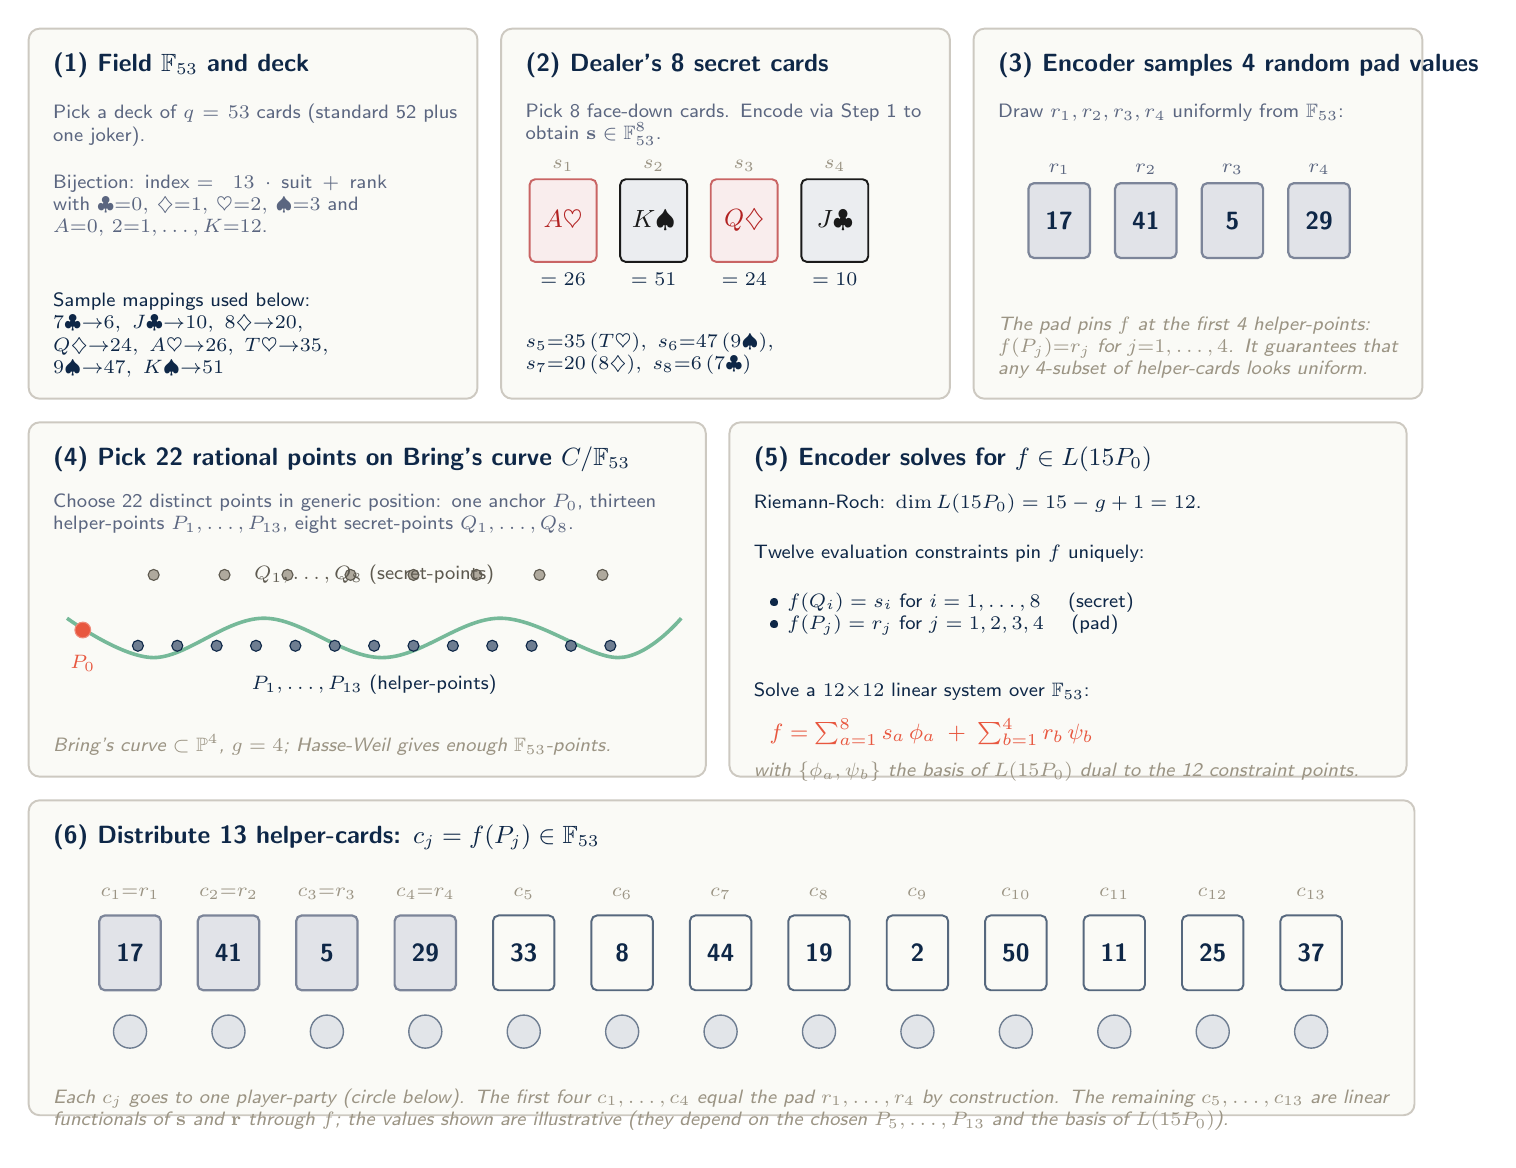
\begin{tikzpicture}[
  panel/.style={
    rectangle, draw=cmuted!50, fill=ccream, rounded corners=4pt,
    line width=0.7pt
  },
  steptitle/.style={cnavy, font=\sffamily\bfseries\small, anchor=north west},
  bodytext/.style={cslate, font=\sffamily\scriptsize, anchor=north west, align=left},
  mathtext/.style={cnavy, font=\sffamily\scriptsize, anchor=north west, align=left},
  redcard/.style={
    rectangle, rounded corners=2pt, draw=cred!70, fill=cred!8,
    line width=0.7pt, minimum width=0.85cm, minimum height=1.05cm,
    inner sep=0pt
  },
  blackcard/.style={
    rectangle, rounded corners=2pt, draw=cblack, fill=cslate!12,
    line width=0.7pt, minimum width=0.85cm, minimum height=1.05cm,
    inner sep=0pt
  },
  padcard/.style={
    rectangle, rounded corners=2pt, draw=cslate!80, fill=cslate!18,
    line width=0.8pt, minimum width=0.78cm, minimum height=0.95cm,
    inner sep=0pt
  },
  helpercard/.style={
    rectangle, rounded corners=2pt, draw=cnavy!70, fill=ccream,
    line width=0.7pt, minimum width=0.78cm, minimum height=0.95cm,
    inner sep=0pt
  },
  player/.style={
    circle, draw=cnavy!60, fill=cnavy!12, line width=0.5pt,
    minimum size=0.42cm, inner sep=0pt
  },
  font=\sffamily
]

% Canvas layout (top-left at (0, 14)):
%   Row 1 (Steps 1-3): y in [9.0, 14.0],  three panels each 5.7 cm wide
%   Row 2 (Steps 4-5): y in [4.3, 9.0],   two panels each 8.6 cm wide
%   Row 3 (Step 6):    y in [0.0, 4.0],   one full-width panel 17.6 cm

% ============================================================
% Row 1: Steps 1, 2, 3
% ============================================================

% --- Panel 1: Field and deck ---
\node[panel, minimum width=5.7cm, minimum height=4.7cm, anchor=north west] (P1)
  at (0.0, 14.0) {};
\node[steptitle] at ($(P1.north west)+(0.20,-0.20)$)
  {(1) Field $\mathbb{F}_{53}$ and deck};
\node[bodytext, text width=5.3cm]
  at ($(P1.north west)+(0.20,-0.85)$)
  {Pick a deck of $q=53$ cards (standard 52 plus one joker).};
\node[bodytext, text width=5.3cm]
  at ($(P1.north west)+(0.20,-1.75)$)
  {Bijection: index $= 13\cdot\text{suit} + \text{rank}$ with
   $\clubsuit{=}0,\,\diamondsuit{=}1,\,\heartsuit{=}2,\,\spadesuit{=}3$
   and $A{=}0,\,2{=}1,\dots,K{=}12$.};
\node[mathtext, text width=5.3cm]
  at ($(P1.north west)+(0.20,-3.25)$)
  {Sample mappings used below:\\
   $7\clubsuit{\to}6,\ J\clubsuit{\to}10,\ 8\diamondsuit{\to}20,$\\
   $Q\diamondsuit{\to}24,\ A\heartsuit{\to}26,\ T\heartsuit{\to}35,$\\
   $9\spadesuit{\to}47,\ K\spadesuit{\to}51$};

% --- Panel 2: 8 secret cards ---
\node[panel, minimum width=5.7cm, minimum height=4.7cm, anchor=north west] (P2)
  at (6.0, 14.0) {};
\node[steptitle] at ($(P2.north west)+(0.20,-0.20)$)
  {(2) Dealer's 8 secret cards};
\node[bodytext, text width=5.3cm]
  at ($(P2.north west)+(0.20,-0.85)$)
  {Pick 8 face-down cards. Encode via Step 1 to obtain
   $\mathbf{s} \in \mathbb{F}_{53}^{8}$.};

% Row 1 of 4 cards (s1..s4)
% Card 1: A heart (red)
\node[redcard] at ($(P2.north west)+(0.80, -2.45)$) {};
\node[cred, font=\sffamily\bfseries\small] at ($(P2.north west)+(0.80, -2.45)$)
  {$A\heartsuit$};
\node[cmuted, font=\sffamily\scriptsize] at ($(P2.north west)+(0.80, -1.75)$)
  {$s_1$};
\node[cnavy, font=\sffamily\bfseries\scriptsize] at ($(P2.north west)+(0.80, -3.20)$)
  {$=26$};
% Card 2: K spade
\node[blackcard] at ($(P2.north west)+(1.95, -2.45)$) {};
\node[cblack, font=\sffamily\bfseries\small] at ($(P2.north west)+(1.95, -2.45)$)
  {$K\spadesuit$};
\node[cmuted, font=\sffamily\scriptsize] at ($(P2.north west)+(1.95, -1.75)$)
  {$s_2$};
\node[cnavy, font=\sffamily\bfseries\scriptsize] at ($(P2.north west)+(1.95, -3.20)$)
  {$=51$};
% Card 3: Q diamond
\node[redcard] at ($(P2.north west)+(3.10, -2.45)$) {};
\node[cred, font=\sffamily\bfseries\small] at ($(P2.north west)+(3.10, -2.45)$)
  {$Q\diamondsuit$};
\node[cmuted, font=\sffamily\scriptsize] at ($(P2.north west)+(3.10, -1.75)$)
  {$s_3$};
\node[cnavy, font=\sffamily\bfseries\scriptsize] at ($(P2.north west)+(3.10, -3.20)$)
  {$=24$};
% Card 4: J club
\node[blackcard] at ($(P2.north west)+(4.25, -2.45)$) {};
\node[cblack, font=\sffamily\bfseries\small] at ($(P2.north west)+(4.25, -2.45)$)
  {$J\clubsuit$};
\node[cmuted, font=\sffamily\scriptsize] at ($(P2.north west)+(4.25, -1.75)$)
  {$s_4$};
\node[cnavy, font=\sffamily\bfseries\scriptsize] at ($(P2.north west)+(4.25, -3.20)$)
  {$=10$};

% Row 2 of 4 cards (s5..s8): compact form on second row not needed; instead show s5..s8 as a math list
\node[mathtext, text width=5.3cm]
  at ($(P2.north west)+(0.20,-3.75)$)
  {$s_5{=}35\,(T\heartsuit),\ s_6{=}47\,(9\spadesuit),$\\
   $s_7{=}20\,(8\diamondsuit),\ s_8{=}6\,(7\clubsuit)$};

% --- Panel 3: 4 pad values ---
\node[panel, minimum width=5.7cm, minimum height=4.7cm, anchor=north west] (P3)
  at (12.0, 14.0) {};
\node[steptitle] at ($(P3.north west)+(0.20,-0.20)$)
  {(3) Encoder samples 4 random pad values};
\node[bodytext, text width=5.3cm]
  at ($(P3.north west)+(0.20,-0.85)$)
  {Draw $r_1,r_2,r_3,r_4$ uniformly from $\mathbb{F}_{53}$:};

% Pad cards row
\foreach \i/\xp/\val in {1/1.10/17, 2/2.20/41, 3/3.30/5, 4/4.40/29} {
  \node[padcard] at ($(P3.north west)+(\xp, -2.45)$) {};
  \node[cnavy, font=\sffamily\bfseries\small] at ($(P3.north west)+(\xp, -2.45)$)
    {\val};
  \node[cslate, font=\sffamily\scriptsize] at ($(P3.north west)+(\xp, -1.80)$)
    {$r_{\i}$};
}

\node[bodytext, cmuted, font=\sffamily\itshape\scriptsize, text width=5.3cm]
  at ($(P3.north west)+(0.20,-3.55)$)
  {The pad pins $f$ at the first 4 helper-points:
   $f(P_j){=}r_j$ for $j{=}1,\dots,4$. It guarantees that
   any 4-subset of helper-cards looks uniform.};

% ============================================================
% Row 2: Steps 4, 5
% ============================================================

% --- Panel 4: Points on Bring's curve ---
\node[panel, minimum width=8.6cm, minimum height=4.5cm, anchor=north west] (P4)
  at (0.0, 9.0) {};
\node[steptitle] at ($(P4.north west)+(0.20,-0.20)$)
  {(4) Pick 22 rational points on Bring's curve $C/\mathbb{F}_{53}$};
\node[bodytext, text width=8.2cm]
  at ($(P4.north west)+(0.20,-0.80)$)
  {Choose 22 distinct points in generic position:
   one anchor $P_0$, thirteen helper-points $P_1,\dots,P_{13}$,
   eight secret-points $Q_1,\dots,Q_8$.};

% Schematic curve drawing (absolute coords: P4.north west = (0, 9.0))
\draw[cgreen!70, line width=1.3pt, smooth, tension=0.6]
  plot coordinates {(0.5,6.5) (1.6,6.0) (3.0,6.5) (4.5,6.0) (6.0,6.5) (7.5,6.0) (8.3,6.5)};

% Anchor P0 (orange)
\node[circle, fill=corange, draw=corange!70, minimum size=0.20cm, inner sep=0pt]
  (PT0) at ($(P4.north west)+(0.7, -2.65)$) {};
\node[corange, font=\sffamily\scriptsize, anchor=north]
  at ($(P4.north west)+(0.7, -2.85)$) {$P_0$};

% 13 helper-points P1..P13 (navy dots)
\foreach \i/\xx in {1/1.4, 2/1.9, 3/2.4, 4/2.9, 5/3.4, 6/3.9, 7/4.4, 8/4.9, 9/5.4, 10/5.9, 11/6.4, 12/6.9, 13/7.4} {
  \node[circle, fill=cnavy!60, draw=cnavy, minimum size=0.14cm, inner sep=0pt]
    at ($(P4.north west)+(\xx, -2.85)$) {};
}
\node[cnavy, font=\sffamily\scriptsize, anchor=north]
  at ($(P4.north west)+(4.4, -3.10)$) {$P_1,\dots,P_{13}$ (helper-points)};

% 8 secret-points Q1..Q8 (muted dots, above curve)
\foreach \i/\xx in {1/1.6, 2/2.5, 3/3.3, 4/4.1, 5/4.9, 6/5.7, 7/6.5, 8/7.3} {
  \node[circle, fill=cmuted!80, draw=cmuted!60!black, minimum size=0.14cm, inner sep=0pt]
    at ($(P4.north west)+(\xx, -1.95)$) {};
}
\node[cmuted!60!black, font=\sffamily\scriptsize, anchor=north]
  at ($(P4.north west)+(4.4, -1.7)$) {$Q_1,\dots,Q_8$ (secret-points)};

\node[bodytext, cmuted, font=\sffamily\itshape\scriptsize, text width=8.2cm]
  at ($(P4.north west)+(0.20,-3.85)$)
  {Bring's curve $\subset \mathbb{P}^4$, $g=4$; Hasse-Weil gives enough $\mathbb{F}_{53}$-points.};

% --- Panel 5: Encoder solves for f ---
\node[panel, minimum width=8.6cm, minimum height=4.5cm, anchor=north west] (P5)
  at (8.9, 9.0) {};
\node[steptitle] at ($(P5.north west)+(0.20,-0.20)$)
  {(5) Encoder solves for $f \in L(15 P_0)$};
\node[mathtext, text width=8.2cm]
  at ($(P5.north west)+(0.20,-0.80)$)
  {Riemann-Roch: $\dim L(15 P_0) = 15 - g + 1 = 12$.};
\node[mathtext, text width=8.2cm]
  at ($(P5.north west)+(0.20,-1.45)$)
  {Twelve evaluation constraints pin $f$ uniquely:};
\node[mathtext, text width=8.2cm]
  at ($(P5.north west)+(0.40,-2.05)$)
  {\textbullet\ $f(Q_i) = s_i$ for $i=1,\dots,8$ \quad (secret)\\
   \textbullet\ $f(P_j) = r_j$ for $j=1,2,3,4$ \quad (pad)};

\node[mathtext, text width=8.2cm]
  at ($(P5.north west)+(0.20,-3.20)$)
  {Solve a $12{\times}12$ linear system over $\mathbb{F}_{53}$:};
\node[corange, font=\sffamily\bfseries\footnotesize, anchor=north west]
  at ($(P5.north west)+(0.40,-3.65)$)
  {$f = \sum_{a=1}^{8} s_a\,\phi_a \;+\; \sum_{b=1}^{4} r_b\,\psi_b$};
\node[bodytext, cmuted, font=\sffamily\itshape\scriptsize, text width=8.2cm]
  at ($(P5.north west)+(0.20,-4.20)$)
  {with $\{\phi_a,\psi_b\}$ the basis of $L(15 P_0)$ dual to the 12 constraint points.};

% ============================================================
% Row 3: Step 6 - distribute 13 helper-cards
% ============================================================

\node[panel, minimum width=17.6cm, minimum height=4.0cm, anchor=north west] (P6)
  at (0.0, 4.2) {};
\node[steptitle] at ($(P6.north west)+(0.20,-0.20)$)
  {(6) Distribute 13 helper-cards: $c_j = f(P_j) \in \mathbb{F}_{53}$};

% 13 helper-cards: c1..c4 = pad (filled slate), c5..c13 computed
\foreach \j/\xp/\val in {1/1.30/17, 2/2.55/41, 3/3.80/5, 4/5.05/29} {
  \node[padcard] at ($(P6.north west)+(\xp, -1.95)$) {};
  \node[cnavy, font=\sffamily\bfseries\small] at ($(P6.north west)+(\xp, -1.95)$)
    {\val};
  \node[cmuted, font=\sffamily\scriptsize] at ($(P6.north west)+(\xp, -1.20)$)
    {$c_{\j}{=}r_{\j}$};
  \node[player] at ($(P6.north west)+(\xp, -2.95)$) {};
}
\foreach \j/\xp/\val in {5/6.30/33, 6/7.55/8, 7/8.80/44, 8/10.05/19, 9/11.30/2, 10/12.55/50, 11/13.80/11, 12/15.05/25, 13/16.30/37} {
  \node[helpercard] at ($(P6.north west)+(\xp, -1.95)$) {};
  \node[cnavy, font=\sffamily\bfseries\small] at ($(P6.north west)+(\xp, -1.95)$)
    {\val};
  \node[cmuted, font=\sffamily\scriptsize] at ($(P6.north west)+(\xp, -1.20)$)
    {$c_{\j}$};
  \node[player] at ($(P6.north west)+(\xp, -2.95)$) {};
}

\node[bodytext, cmuted, font=\sffamily\itshape\scriptsize, text width=17.0cm]
  at ($(P6.north west)+(0.20,-3.55)$)
  {Each $c_j$ goes to one player-party (circle below). The first four
   $c_1,\dots,c_4$ equal the pad $r_1,\dots,r_4$ by construction. The
   remaining $c_5,\dots,c_{13}$ are linear functionals of $\mathbf{s}$ and
   $\mathbf{r}$ through $f$; the values shown are illustrative
   (they depend on the chosen $P_5,\dots,P_{13}$ and the basis of $L(15 P_0)$).};

\end{tikzpicture}
\end{document}
